\chapter{Problem Solution}\label{chap:problem-solution}

\section*{}

In this chapter, a preliminary approach for the problem defined in the previous chapter is presented. In some cases, it is still not possible to make a clear decision, as it requires implementation and further testing to validate that it actually works, and really fits the need. These proposed approaches are based on the research done in the Chapter \ref{chap:sota}, projected into the application domain and specific needs. This chapter is divided in three sections, which will more precisely elaborate on their respective topic, presenting one or multiple proposed solutions for that specific area. 

\section{Knowledge Base}
This project will benefit of the existing structure of zerozero.pt knowledge base, and will integrate with it, by pulling events data from it, as well as publishing the event inputs generated by the users, storing the event history.

\section{High Level Architecture}

Fig. \ref{fig:high-level-arch} presents the proposed high level design for the application. The ZeroZero API is already available. The relevant parts are the ZeroZero Live Web Server, which will serve the web pages to the clients, mediating the state synchronization among them. It will communicate with the existing ZeroZero API for authentication and access to existing event information. It will also communicate with other two micro-services. Reputation Service will handle the reputation calculation regarding the interactions during the event. Conflict Handling Service is responsible for handling the conflicts in real time, resolving them automatically whenever possible and cleaning up the event state. The Web clients will contain the frontend web pages with the logic to store changes locally and allow for offline working, as well as listening for the real-time updates to keep the state synchronized.

\begin{figure}[t]
    \begin{center}
        \leavevmode
        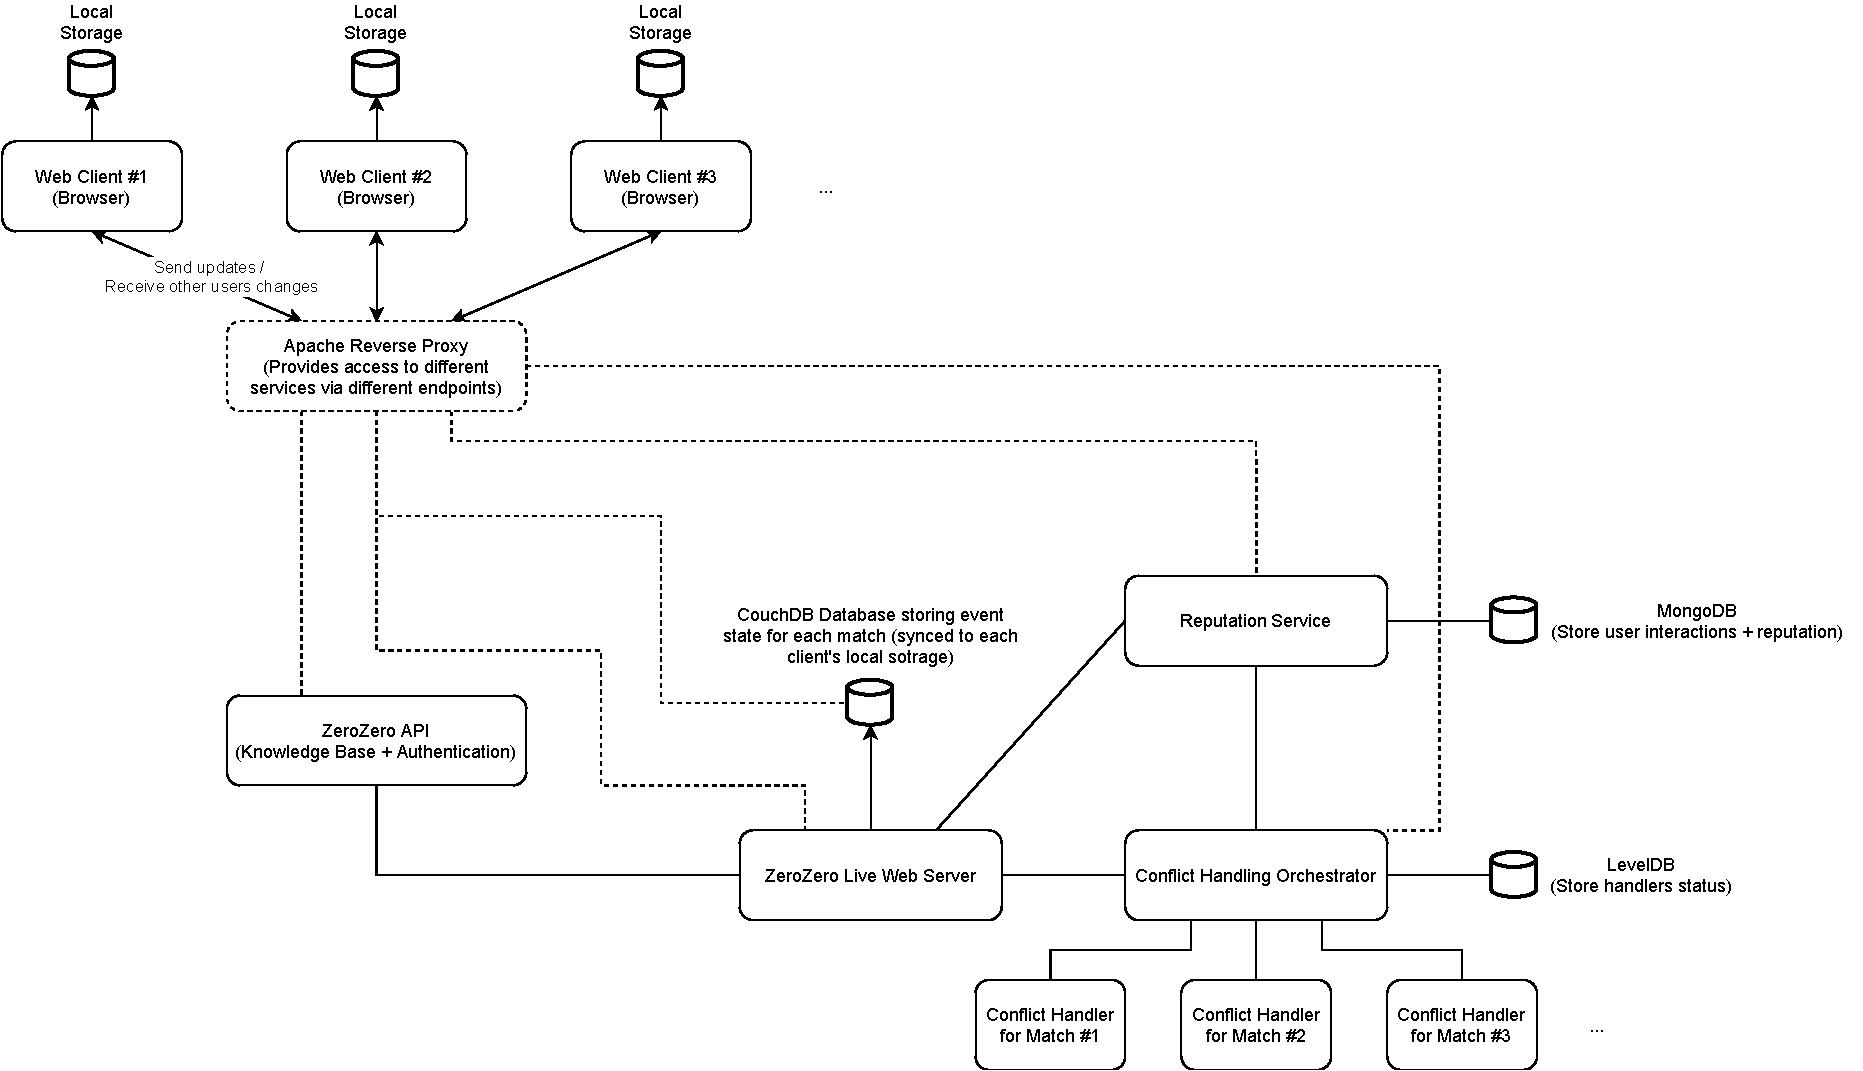
\includegraphics[width=0.9\textwidth]{zerozerolive-arch.pdf}
        \caption{High Level Architecture design of the zerozero.live system}
        \label{fig:high-level-arch}
    \end{center}
\end{figure}

\section{Offline Availability} \label{sec:prob-solution-offline-avail}
According to the research done in Chapter \ref{chap:sota}, there needs to be a way of storing state locally, in case the user is offline. Since, this application is a web application, from the alternatives presented, \textbf{localStorage} seems to be the most available among browsers\footnote{https://caniuse.com/?search=localstorage}, while fitting the project's needs. 

Currently, in the already existing \say{Proof-of-Concept}, there is an already implemented solution, which uses a local queue of requests stored in \textit{localStorage}, so as to not overwhelm the server with changes every second. This queue is \say{dumped} every 10 seconds, that is, every 10 seconds, the operations batched in the queue are sent to the server. While this allows for prevention of operations loss in case of sudden network connectivity, it might not be the best approach in terms of real-time and user experience. For example, let's say that a user generates a conflicting operation, but that operation is only sent 10 seconds later. Only then the user will see that effect on is device, when it could have happened sooner.

My proposal is to reduce the waiting time to a more reasonable 2 seconds, which, while preventing the overwhelming of messages to the server, reduces notification time and still lets the user cancel the operation before it being sent.

\section{Conflict Resolution} \label{sec:prob-solution-conflict-res}
This is a topic on which there is no clear solution. As it was seen in the research, the most well-know and used approaches are OT and CRDT. The community cannot, however, elect a clear winner\footnote{https://news.ycombinator.com/item?id=22039950}, they are just \textit{different}. On the OT side, a common approach is to use ShareDB\footnote{https://github.com/share/sharedb}, together with the JSON OT type definition\footnote{https://github.com/ottypes/json0}.

Another alternative would be to use CouchDB\footnote{https://couchdb.apache.org/} with its web browser counterpart, PouchDB\footnote{https://pouchdb.com/}. It allows for replication of state among all users, with complete control on conflict resolution: When CouchDB encounters a conflict scenario, it arbitrarily chooses a winner, deterministically, however, it keeps the conflicting version as well, which can be used to solve the conflict with custom application logic, for example, based on a reputation system, or on merging the two inputs --- Creative Resolution (Section \ref{sec:conflict-res-sota})

On the CRDT side, there are two options: Automerge\footnote{https://github.com/automerge/automerge} and GUN\footnote{https://github.com/amark/gun}. Since the latter's documentation seems to be lacking, I am removing it from the options pool. Automerge is flexible enough, allowing for server-client network architecture, as well as peer-to-peer, and it works like JSON CRDT were described to work: each user has a local copy of the JSON state, which can be locally mutated, even when offline, and it will sync automatically with other nodes. It works similarly to the CouchDB/PouchDB conflict handling, in being as much automatic as possible, but letting the application know about existing conflicts and handle them.

At this point, the ShareDB option seems to work on a lower level than the other two, and it might be unfeasible to have good results in the expected timeframe. Between CouchDB/PouchDB and Automerge, there is no clear winner, the only distinctive charateristic being that CouchDB is more mature and has been used in production for much longer. Nevertheless, the wise decision here would be to try both in a small \say{Proof-of-Concept} and further verify their usability. 

\section{Reputation System} \label{sec:problem-solution-rep-sys}
As was mentioned in the Literature Review (Section \ref{sec:rep-sys-sota}), an effective method to achieve a fair reputation system, which takes into account the time dynamics of user interactions as well as their current reputation, is to implement a personalized PageRank algorithm, which takes into account the reputation of users when calculating vouching or invalidation, in order to achieve a weighted voting system so as to provide long-term reputable users with a prize for their good behavior. Recalling the system present in \cite{Daly2009}, there are 4 rules involved in adapting the system to our use case:

\begin{enumerate}
    \item Every time a user consumes a document from an author, the author gains reputation;
    \item Every time a user consumes a document, the document gains \say{reputation} (i.e. popularity);
    \item In order to take time dynamics into account, reputation should decrease over time, so that a \say{rich-get-richer} paradigm can be avoided (both for users and for documents);
    \item Users with higher reputation matter more when calculating the document reputation changes;
\end{enumerate}

With this in mind, I propose the following rules to adapt this to our scenario:

\begin{itemize}
    \item Every time a user agrees with an input, he will improve the input's reputation according to rules 2 and 4;
    \begin{multline}
        newInputRep = oldInputRep + (1 - oldInputRep) * maxRepReward * userRep\\ * userRepInfluence
    \end{multline}
    \item Every time a user disagrees with an input (either by inputting a real-conflicting input or reporting as false/inaccurate) he will worsen the input's rep according to rules (2's reverse) and 4;
    \begin{equation}
        newInputRep = oldInputRep * (1 - maxRepPunishment * userRep * userRepInfluence)
    \end{equation}
    \item Every time a user submits a falsely-conflicting input, meaning that both users submitted the same information resulting in duplicated information, it should act as an explicit agreement with the other user's input, so it should count more, according to an $explicitAgreementBonus$ constant, which must be greater than zero to achieve the bonus effect;
    \begin{multline}
    newInputRep = oldInputRep \\+ ((1 - oldInputRep) * repReward * userRep * userRepInfluence)\\ * (1 + explicitAgreementBonus)
    \end{multline}
    \item The user gains reputation according to the average of its inputs' reputations. Only takes into account the latest inputs, referring to the last event which will trigger the reputation update;
    \begin{equation}
        newUserRep = oldUserRep + (1 - oldUserRep) * \frac{\sum inputRep}{numInputs}
    \end{equation}
    \item Each user has a reputation decay according to rule 3, the time unit should be 1 week since there's at least one relevant game per week. This prevents users that generate a lot of inputs in a single game to enjoy their reputation boost for many more games, since they need to be consistent every week: it matters more if they make an input every week than 20 inputs once every 2 or more weeks.
    This decay is on a higher level than the events, creating 20 inputs in an event is roughly the same as 1 input in an event (since the football events last around 90 minutes)
    \begin{equation}
        newUserRep = oldUserRep * decayCoefficient^{timeSinceLastUpdate}
    \end{equation}
    \item The reputation values are updated at the end of each event, according to the event's history.
\end{itemize}
